%\documentclass[journal,draftcls,onecolumn,12pt,twoside]{IEEEtranTCOM}
%\documentclass[journal,twocolumn,twoside]{IEEEtran}
%\documentclass[journal,twocolumn,12pt,twoside]{IEEEtranTCOM}
\documentclass[journal]{IEEEtran}
\usepackage[latin1]{inputenc}
\usepackage[dvips]{graphicx}
\usepackage{subfig}
%\usepackage{eps2pdf}
\usepackage{epsfig}
%\usepackage{amssymb}
%\usepackage[cmex10]{amsmath}
\usepackage{mdwmath}
\usepackage{eqparbox}
\usepackage{amsbsy}
\usepackage{cite}
\usepackage{amsmath,amsfonts,amssymb,amstext}
\usepackage{dsfont}
\usepackage{blindtext} %para gerar textos "lorem ipsum" - \blindtext


%*** Meus Pacotes **********************************
\usepackage{enumerate}
\usepackage{psfrag}
\usepackage{graphicx,color}               %para habilitar letras coloridas
%Cria um comando para alerta de necessidade de revisão
\newenvironment{rev}[1]{\textcolor{red}{\bf(REVISAR)} \textcolor{blue}{\bf #1}}

% *****  Definição da lista de Símbolos  *****
\renewcommand{\Re}{\mathrm{Re}}                    %"parte real"
\renewcommand{\Im}{\mathrm{Im}}                    %"parte imaginária"
\renewcommand{\emptyset}{\mbox{\large{\o}}}        %"conjunto vazio"

%\newcommand{\diag}{\mathrm{diag}}                  %diag{}
%\newcommand{\W}{\mbox{\bf $\mathcal{W}$}}          %variável do equalizador
%\newcommand{\HH}{\mbox{\bf $\mathcal{H}$}}         %matriz de convolução do canal
%\newcommand{\btil}[1]{\mathbf{\widetilde{#1}}}     %variável de matriz
%\newcommand{\bhat}[1]{\mathbf{\widehat{#1}}}       %variável de matriz
%\newcommand{\F}{\mbox{\bf $\mathcal{F}$}}          %matriz de Fourier
%\newcommand{\vet}[1]{\mbox{$\boldsymbol{#1}$}}     %negrito de letras minúscuas Gregas


% Siglas
\usepackage{acronym}
\newacro{PLC}{power line communication}
\newacro{OFDM}{orthogonal frequency division multiplexing}
\newacro{HS-OFDM}{Hermitian symmetric orthogonal frequency division multiplexing}
\newacro{IP}{internet protocol}
\newacro{QoS}{quality of service}
\newacro{UFJF}{Universidade Federal de Juiz de Fora}
\newacro{LIT}{linear e invariante no tempo}
\newacro{LVT}{linear e variante no tempo}
\newacro{LPVT}{linear e periodicamente variante no tempo}
\newacro{CIR}{channel impulse response}
\newacro{CFR}{channel frequency response}
\newacro{ACFR}{average channel frequency response}
\newacro{LV-PDN}{low voltage power distribution network}
\newacro{RMS-DS}{root-mean-square delay spread}
\newacro{CB}{coherence bandwidth}
\newacro{CT}{coherence time}
\newacro{DAC}{digital-to-analog converter}
\newacro{ADC}{analog-to-digital converter}
\newacro{SNR}{signal-to-noise ratio}
\newacro{SEE}{signal energy estimation}
\newacro{ISI}{inter symbol interference}
\newacro{WSSUS}{wide-sense stationary uncorrelated scattering}
\newacro{ACM}{average channel magnitude}
\newacro{ACG}{average channel gain}
\newacro{ACA}{average channel attenuation}
\newacro{CDF}{cumulative distribution function}
\newacro{PSD}{power spectral densities}
\newacro{ADR}{achievable data rate}

\newcommand{\tamfig}{3.5in}    %\newcommand{\LARGURA}{12cm}         %largura das figuras Matlab

\normalsize
% correct bad hyphenation here
\hyphenation{op-tical net-works semi-conduc-tor}


\begin{document}

\title{Top-Down Characterization of Low Voltage Electric Power Distribution Networks for Use of PLC Systems}

\author{Antonio~A.~M.~Picorone,
        Thiago~R.~Oliveira,  
        Raimundo~Sampaio-Neto,~\IEEEmembership{Senior~Member,~IEEE,}     
        and~Moises~V.~Ribeiro,~\IEEEmembership{Senior~Member,~IEEE}% <-this % stops a space

 \thanks{A. A. M. Picorone (antonio.picorone@ufjf.edu.br) is with the Production Engineering and Mechanics Department, Federal University of Juiz de Fora (UFJF), Juiz de Fora, Brazil.}% <-this % stops a space
 \thanks{T. R. Oliveira (thiago.oliveira@ifsudestemg.edu.br) is with the Electronics Department, Federal Institute of Education, Science and Technology of the Southeast of Minas Gerais (IFSEMG), Campus Juiz de Fora, Brazil.}% <-this % stops a space
 \thanks{R. Sampaio-Neto (raimundo@cetuc.puc-rj.br) is with the Pontif\'icia Universidade Cat\'olica do Rio de Janeiro (PUC-RJ), Rio de Janeiro, Brazil.}% <-this % stops a space
\thanks{M. V. Ribeiro (mribeiro@ieee.org) is with the Electrical Engineering Department,
Federal University of Juiz de Fora (UFJF), and Smarti9 Ltda, Brazil.}% <-this % stops a space
}

% The paper headers
\markboth{Electric Power Systems Research}%
{Submitted paper}

\maketitle

\begin{abstract}
This paper presents unprecedented results of a comprehensive measurement campaign based on sounding approach with the aim of characterizing and modeling the outdoor Brazilian as a means of data communication. Average channel attenuation, root-mean-square delay spread, coherence time, coherence bandwidth and achievable data rate are analyzed in the frequency band from 1.7 MHz up to 100 MHz. Statistical models for some channel features are proposed. The cyclically periodic variation of the channel is quantified and presented as a temporal function of the average channel attenuation variation. Also, mathematical models based on only two parameters representing both the background and impulsive noises are proposed. The parameters analyzed in this contribution can help the characterization of outdoor Brazilian power line channels, since increase the knowledge about such communication media, contributing to the design of increasingly robust and efficient PLC systems.
\end{abstract}

\begin{IEEEkeywords}
power line communication, channel estimation, statistical modeling, channel features.
\end{IEEEkeywords}
\acresetall
%\IEEEpeerreviewmaketitle

\section{Introduction}\label{sec:intro}
\IEEEPARstart{T}{he} development of data communication systems capable of interconnecting the most diverse electro-electronic devices has motivated many researchers lately. Smart cities \cite{Andrisano2018}, smart buildings \cite{Minoli2017} and smart grids \cite{Masera2018} are examples that can only be realized through a communication network that integrates existing technologies in homes, in vehicles, in commerce, in the electric power network, etc. Furthermore, much of this integration has been discussed within concept of Internet of Things (IoT) \cite{Atzori2010}. On the other hand, nowadays there is no single technology that meets all requirements necessary for the interconnection of the present devices, given the diversity and complexity of the environments to be integrated. Consequently, there are combinations of a wide variety of communication systems that are used for this purpose \cite{Mehmood2017, M.B.A.Dib2018}.

When smart grids are considered, \ac{PLC} emerges as a natural choice largely evaluated in the literature \cite{Yan2013, Han2017, Artale2018}. One of the great motivations of the use of this technology lies in the infrastructure that has already been installed and its great potential for network convergence \cite{Willie2006,M.B.A.Dib2018,Oliveira2017}. Though \ac{PLC} is potentially convenient for low-cost data transmission for measurement and control of electricity supply, water and gas consumption, and in industries, the electric power grids constitute a challenging medium for data communication since they were not designed for this purpose \cite{Corripio2006,Musolino2008,Zimmermann2000}. In order to design an efficient communication system, regardless the type of system, the knowledge of the effects that a communication signal is subjected through its propagation in the communication medium is mandatory. This effects are usually evaluated as a function of some channel parameters, such as \ac{ACA}, \ac{RMS-DS}, \ac{CB}, and \ac{CT}.    

The propagation characteristics of \ac{PLC} signals in indoor low voltage networks are well-known in the literature \cite{Zimmermann2002, Tlich2008, Tlich2008a, Tonello2014}, due mainly to the ease physical access to the networks. On the other hand, although knowledge of medium characteristics is extremely important, papers with a focus on \ac{LV-PDN} are not common in the literature, due mainly to the complexity of conducting measurement campaigns in these environments. In \cite{Liu2000} a measurement campaign was carried out in Germany. In that work, the \ac{ACA}, noise, and \ac{RMS-DS} of the \ac{PLC} outdoor channels (\ac{LV-PDN}) in the 1~MHz up to 30~MHz frequency band were evaluated. The results of a small measurement campaign was presented in \cite{Prasad2001} and aimed to characterize the \ac{LV-PDN} for outdoor \ac{PLC} communication in India. The results reported in \cite{Prasad2001} are also restricted to the frequency band from 1~MHz up to 30~MHz and evaluated the \ac{ACA}, \ac{RMS-DS} and \ac{CB}. For outdoor \ac{PLC} channels, \cite{Liu2000} reported values of 1.4~$\mu$s  considering a single frequency of 3.75~MHz and of 0.8~$\mu$s for the 5~MHz frequency. However, it has not been clearly defined whether these values represent \ac{CIR} duration or the \ac{RMS-DS} value. Values of \ac{RMS-DS} between 0.145~$\mu$s and 0.228~$\mu$s in the frequency range of 1.7~MHz up to 30~MHz were reported by \cite{Prasad2001}.

In general, the behavior of \ac{LV-PDN} when used as a data communication medium is not yet well-known. In order to contribute to mitigate this gap, this work aims to increase the scientific knowledge about the characteristics of LV-PDV as a means of data communication. Towards this end, the main contributions of this paper are summarized as follows:
\begin{itemize}
	\item Results of an extensive measurement campaign conducted in the outdoor Brazilian \ac{LV-PDN} are presented with the objective of helping to characterize these networks as a means of \ac{PLC} communication. The measurement campaign was carried out during 14 days in two distinct districts of the city of Juiz de Fora, MG, Brazil;	 
	\item Results are presented of numerical analyzes performed on the data obtained from the measurement campaign that help the characterization of \ac{LV-PDN} as a \ac{PLC} communication medium.  The analyzed channel features are \ac{ACA}, \ac{RMS-DS}, \ac{CB}, \ac{CT}, and \ac{ADR};
	\item The background and impulsive noises observed in the measurement campaign of outdoor Brazilian \ac{LV-PDN} are analyzed and presented. 
\end{itemize}


Based on numerical analyses, we state the following remarks:
\begin{itemize}
	\item It was observed and quantified the time window occupied by the abrupt \ac{ACA} variation due to the cyclic switching of charges synchronized with the electric power network. Statistically, \ac{RMS-DS} presents values following, with good approximation, the inverse Gaussian probability distribution; 
	\item The \ac{CB} presents values following, with good approximation, a inverse Gaussian probability distribution;
	\item Only in 20\% of the analyzed cases the \ac{CT} was less than, approximately, 2~ms for $\beta = 0.99$ and 5~ms for $\beta = 0.95$. The \ac{CT} was not lower than 1.38~ms and 5.76~ms, for $\beta=0.99$ and $\beta = 0.90$, respectively.
\end{itemize}

%The results and analyzes are supported by a wide measurement campaign carried out in the \ac{LV-PDN} in the city of Juiz de Fora, Brazil, in order to explore the use of communication systems based on outdoor \ac{PLC} technology. The analyzed channel features are \ac{ACA}, \ac{RMS-DS}, \ac{CB}, \ac{CT} and \ac{ADR}.
%The main contributions of the present investigation are summarized as follows:
%\begin{itemize}
%	\item Some data sets presented (\ac{RMS-DS} and \ac{CB}) were modeled by a statistical distribution in which case several classical continuous distributions are considered;
%	\item Adherence tests were conducted by evaluating the associated log-likelihood values, which is the adopted metric to support the choice of the best statistical distribution that models such channel parameter;
%	\item The average duration of the time window occupied by abrupt \ac{ACA} variation of measured outdoor PLC channels was in the first time estimated. Also a robust linear approach of the \ac{ACA} based on the mean square error criterion was presented;
%	\item A robust approach of the mean measured PLC channel attenuation response based on the mean square error criterion was presented;
%	\item The relationship between ACA and RMS-DS, RMS-DS and CB in outdoor \ac{PLC} channel were modeled by robust linear approach based on the mean square error criterion; 
%	\item A mathematical model, based on performed measurements of the noise \ac{PSD} in the \ac{PLC} outdoor communication medium was proposed and the \ac{ADR} of the outdoor PLC channel in the presence both impulsive and background noise was estimated.
%\end{itemize}

The rest of paper is organized as follows: Section \ref{sec:campaign} the measurement setup and campaign are presented. Section \ref{sec:parameters} parameters used to channel characterize are defined. The results of measurement campaign are presented in the Section \ref{sec-caracteristicas_canal_outdoor}. Finally, the conclusions of this study are presented in Section \ref{sec-conclusao}.

\section{Measurement Setup and Campaign}
\label{sec:campaign}

The statistical characterization and modeling of the features associated with Brazilian outdoor PLC channels were supported by estimates of \ac{CFR}. The data used to estimate the CFR were produced by a set of measurement equipment during a measurement campaign in the city of Juiz de Fora, MG, Brazil, as discussed bellow.

\subsection{Measurement Setup}

The block diagram of the adopted measurement setup applied in order to estimate the \ac{CFR} is depicted in Fig.~\ref{fig:setup} and consists of three main components:
\begin{enumerate}[(i)]
\item Signal generator: Device composed of an arbitrary signal generator board mounted in a rugged computer.
A pre-designed sounding sequence is loaded into it and converted to an analog signal to be submitted to the electric power grid under analysis;
\item Data digitizer: Acts as a receiver, measuring the transmitted sounding signal after propagating through the electric power grid,
and converts it into a digital representation for the subsequent analyzes that will be carried out through digital signal processing-based techniques;
\item Coupler: Circuitry applied to connect both the signal generator and data digitizer to the electric power grid under analysis.
The coupler is essentially composed of an analog high pass filter, blocking the main voltage signal ($60$~Hz in Brazil) that can damage the other equipments \cite{SilvaCosta2017}. Insertion loss lower than 2~dB in the frequency band between 1.7~MHz up to 100~MHz is introduced by adopted coupler.
\end{enumerate}

The set of equipment and algorithms used to inject the test signal into the \ac{LV-PDN} is called Setup TX. On the other hand, the set of equipment and algorithms used to sample and estimate the \ac{LV-PDN} \ac{CFR} is denominated Setup RX.

\begin{figure}[htb]
\begin{centering}
    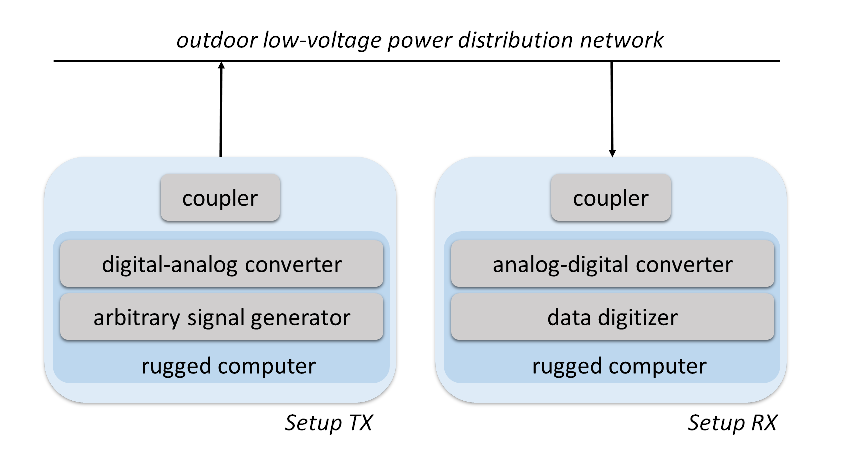
\includegraphics[scale=.6]{Figuras/setups.eps}
    \caption{Block diagram of the measurement setup.}
    \label{fig:setup}
\end{centering}
\end{figure}

The \ac{CFR} estimates were obtained through the estimation methodology described in~\cite{Oliveira2014}, which is based on a sounding approach \cite{Parsons1991}. The set of adopted parameters in the estimation methodology is summarized in Tab.~\ref{tab:setup_parameters}.
Essentially, the transmitted signal is composed of \ac{HS-OFDM} symbols \cite{Ribeiro2014a}. By adopting  $200$~MHz sampling frequency, the frequency resolution is around $48.83$~kHz and each \ac{CFR} estimate is obtained every $23.04~\mu$s, approximately -- for more details see~\cite{Oliveira2013a}. 

\subsection{Measurement Campaign}
For the analysis of the features of the outdoor PLC channel, 33 cycles of the \ac{LV-PDN} fundamental frequency (60~Hz in Brazil) were considered at distinct points in a low-income neighborhood of the city of Juiz de Fora, MG, Brazil. The distance between the couplers ranged from 3~m up to 100~m, with mean values of 15~m, 50~m and 85~m. In each cycle of the \ac{LV-PDN} (16.67~ms), approximately 723 PLC channel frequency responses were collected with a length of 4,096 samples per CFR, in addition to the cyclic prefix of size equal to 512. With this, 23,919 CFR measurements of outdoor PLC channels were evaluated in total.

The measurement of the noise in the outdoor PLC channel was performed according to \cite{Andrade2013}, in which groups of 3,500,000 successive samples of voltage in the time domain of the signal on the \ac{LV-PDN} were obtained in the absence of signal emitted by the signal generator. Each sample group corresponds to approximately 17.5~ms. This time was chosen based on the memory capacity of the data acquisition board when set to a sampling rate of 200~Msps. These samples were acquired in one of the three phases of the \ac{LV-PDN} and form the database of outdoor PLC channel noise.

\begin{table}[!htp]
\centering
  \caption{Main parameters adopted for the CFR estimation.}
  \label{tab:setup_parameters}
\begin{tabular}{c|c}
\hline\hline
Description&Value\\
\hline\hline
Sampling frequency&$f_s=200$~MHz\\
\hline
Number of sub-carriers  &$N=2,048$ \\
\hline
Modulation         &BPSK \\
\hline
Cyclic prefix length       &$L_{cp}=512$ \\
\hline
Frequency resolution&$\Delta_f = 48.83$~kHz\\
\hline
Symbol duration & 23.04 $\mu$s \\
\hline
Length of the sequence $\{y_{j}[n]\}$    &$L_{j}=9,216$ \\
\hline
Number of samples used to compute $\textbf{m}_{t}$     &$K_{d}=8$ \\
\hline
Number of shift in the vector $\textbf{m}_{t}$  calculus       &$R=128$ \\
\hline
\end{tabular}
\end{table}


Figs. \ref{Fig:setupTX} and \ref{Fig:setupRX} illustrate the complex task of installing the setups used as transmitter and receiver in a part of the measurement campaign.
\begin{figure}[!htp]
	\begin{centering}
		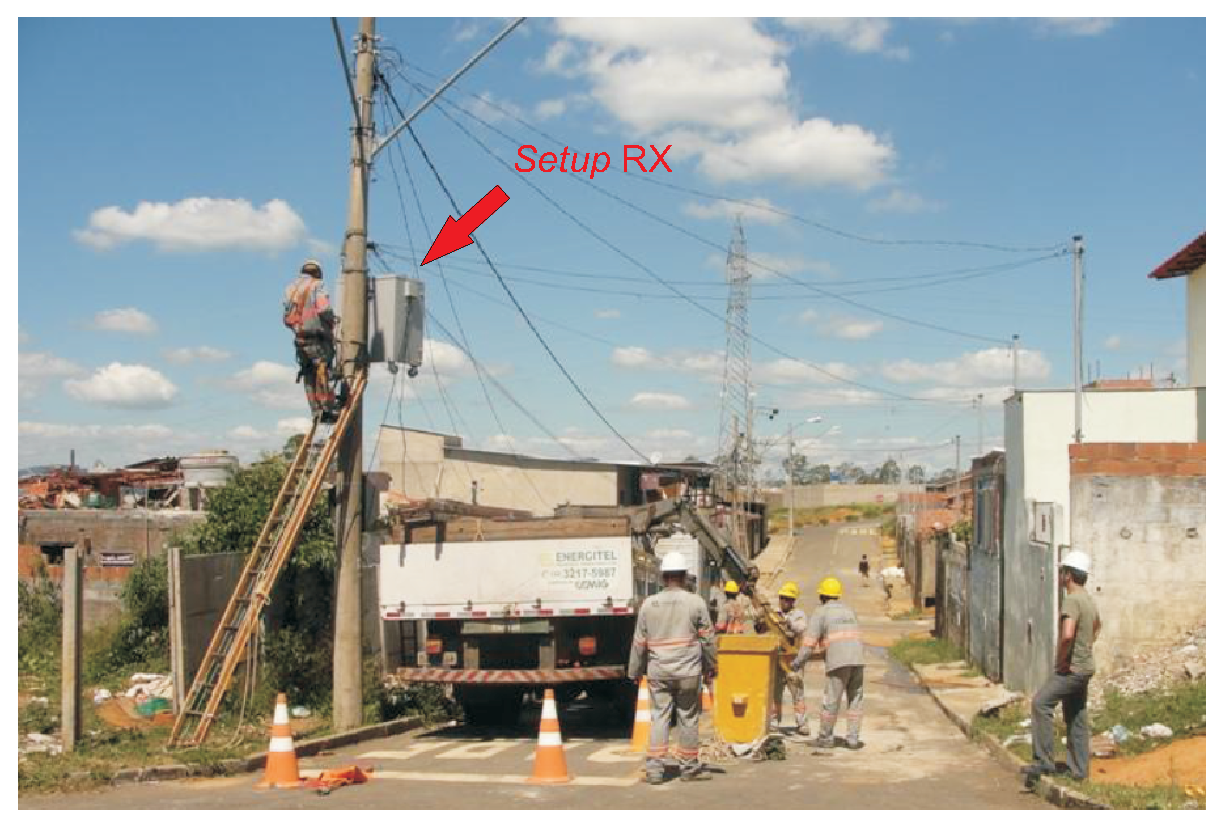
\includegraphics[scale=.4]{Figuras/setupRXnoposte.eps}
		\caption{Setup RX installed on the \ac{LV-PDN} pole.}
       \label{Fig:setupTX}
     \end{centering}
 \end{figure}
 
\begin{figure}[!htp]
	\begin{centering}		
	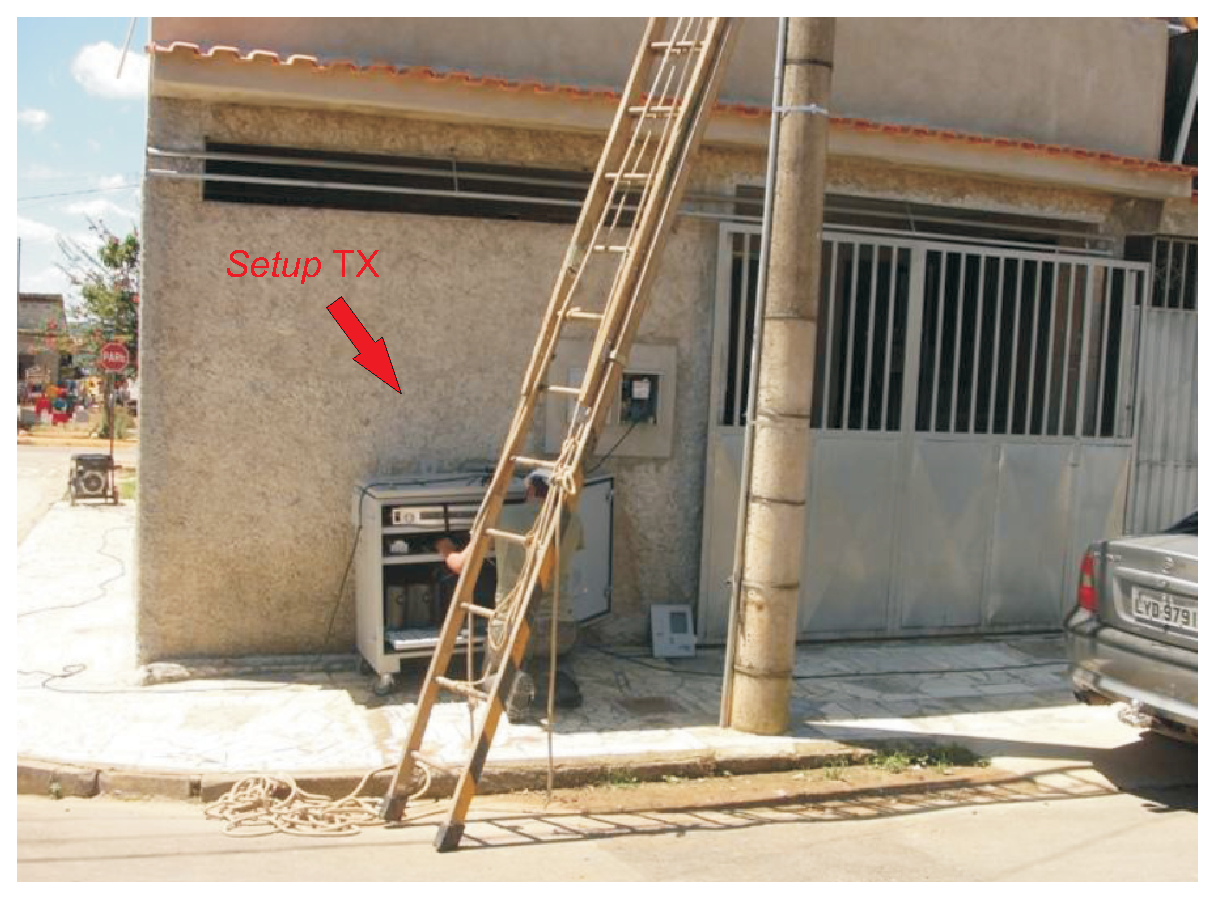
\includegraphics[scale=.4]{Figuras/setupTXnoconsumidor.eps}
	\caption{Setup TX installed near the consumer's electric power meter.}
		\label{Fig:setupRX}
	\end{centering}
\end{figure}

\section{Features Definitions}
\label{sec:parameters}

Let us assume the PLC channels are modeled as band limited and frequency selective \ac{WSSUS}. Also, assume that during a certain period of time, the \ac{CIR} is time-invariant. Therefore, the \ac{CIR} of the \ac{PLC} channel is during this certain time interval is  $ h(t)\in \mathbb{R}|t\in[0,T_h)$,  and its corresponding Fourier transform is $H(f)\in \mathbb{C}||f|<B$, in which $B$ is the frequency bandwidth. Note that $h[n]=h(t)|_{t=nT_s}$, in which $n=0,1.2,\cdots,L_h-1 $ and $T_s$ is the sampling period. The features extracted from the Brazilian PLC channels are described in the following subsections. This assumption is taken into account to define \ac{ACA}, \ac{ACFR}, \ac{RMS-DS}, \ac{CT} and \ac{CB}.

\subsection{Average Channel Attenuation}
The ACA in dB is expressed by
\begin{eqnarray}
	\textrm{ACA}=-10\log_{10}\left(\frac{1}{N}\sum_{k=0}^{N-1}|H[k]|^2\right) \ \ \ \mbox{[dB]},
\end{eqnarray}
where $H[k]$ is the $k^{\rm th}$ coefficient of the discrete channel frequency response for the zero-padded version of the discrete-time impulse response of the time invariant PLC channel $\{h[n]\}_{n=0}^{L_h-1}$ because $L_h \ll N$.


\subsection{Average Channel Frequency Response}
The \ac{ACFR} represents the mean of all measured \ac{CFR} in the measurement campaign carried out, it is expressed by
\begin{eqnarray}
\overline{A}_f=20\log_{10}\left[E\{|H[k]|\}\right] \ \ \ \ \ \mbox{[dB]},
\end{eqnarray}
where $E\{\cdot\}$ denotes the expectation operator.

\subsection{Root Mean Squared Delay Spread}
The RMS-DS represents the distribution of the transmitted power over various paths in a multipath environment,
and can be defined as the square root of the second central moment of a power delay profile.
For a discrete-time channel impulse response, the RMS-DS ($\sigma_{\tau}$) is expressed as
\begin{eqnarray}
	\sigma_{\tau}
	= T_{s}\sigma_{0}
	= T_{s}\sqrt{\mu{}_{0}^{'}-\mu_{0}^{2}},
\end{eqnarray}
where
\begin{eqnarray}
	\mu_{0}=\frac{\overset{L_h-1}{\underset{n=0}{\sum}}n|h\left[n\right]|^{2}}{\overset{L_h-1}{\underset{n=0}{\sum}}|h\left[n\right]|^{2}}\
	~~ {\rm and} ~~
	\mu_{0}^{'}=\frac{\overset{L_h-1}{\underset{n=0}{\sum}}n^{2}|h\left[n\right]|^{2}}{\overset{L_h-1}{\underset{n=0}{\sum}}|h\left[n\right]|^{2}},
\end{eqnarray}
and $T_s=1/f_s$ is the sampling period.
Note that $\sigma_{0}$ is the RMS-DS normalized to a unitary sampling time,
$\mu_{0}$ is the average delay
and $h[n]$ is the $n^{\rm th}$ sample of the discrete-time channel impulse response. The channel impulse response is evaluated over the support of the channel impulse response in the discrete-time domain.

\subsection{Coherence Bandwidth}
The coherence bandwidth reflects how selective the channel frequency response is, being determined by
\begin{eqnarray}
	R(e^{j\omega})=\int_{-\pi}^{\pi} H(e^{j\omega})H^*(e^{j\omega+\Delta\omega})d \omega,
	\label{eq:CB}
\end{eqnarray}
in which $H(e^{j\omega})$ is the Fourier transform of the discrete-time representation of a linear and time invariant PLC channel and  $0 \leq \Delta \omega \leq 2\pi$ denotes the angular frequency resolution in the transform domain. The value of the coherence bandwidth ($\Delta \omega_{B_c}$) in the discrete-time domain is such that
\begin{eqnarray}
|R(e^{j\Delta \omega_{B_c}})|=\gamma|R(1)|,
\label{eq:CB}
\end{eqnarray}
where $0<\gamma<1$ is the correlation level informing that the channel frequency response does not vary considerably when $\Delta \omega \in [0,\Delta \omega_{B_c}]$. Assuming a sampling frequency equal to $f_s=2B$~Hz, in which $B$ is the frequency bandwidth, then the coherence bandwidth ($B_c$) is expressed as
\begin{eqnarray}
B_c=\frac{\Delta \omega_{B_c}}{2\pi}f_s.
\label{eq:CB}
\end{eqnarray}
The CB estimates from the measured PLC channels are analyzed with respect to the correlation coefficient $\gamma = 0.9$. 

\subsection{Coherence Time}
The coherence time is the time duration in which the channel impulse response of a PLC channel is considered time invariant. Following~\cite{Picorone2014}, the evaluation of the coherence time may be carried out by assuming that the PLC channel is an \ac{WSSUS} process. Then, the coherence time of the channel is related to the coherence time of the complex gains of the channel, $\alpha_l(t)$, which incorporate both attenuation and phase deviations due to $l = 1,2,\ldots,L$ multiple reflections of the signal in the communication medium.  

In its turn, the coherence index between samples of $\alpha_l(t)$, taken $\Delta t$ time units apart, is given by
\begin{eqnarray}\label{eq-correlindex}
\rho_{\alpha_l}=\frac{E[\alpha_l(t)\alpha^*_l(t+\Delta t)]}{E[|\alpha_l^2(t)|]},
\end{eqnarray}
in which $E[.]$ is the expectation operator and $*$ denotes the conjugate operator. 
Thus, it can be assumed that the correlation index of the PLC channel is given by
\begin{eqnarray}\label{eq-correl}
\rho_{h}(\Delta t)=\frac{\sum_{l=1}^L P_l \rho_{\alpha_l}(\Delta t)}{\sum_{l=1}^L P_l}; \ \ 0\leq |\rho_h(\Delta t)|\leq 1,
\end{eqnarray}
where $P_l= E[|\alpha_l^2(t)|]$ is the average power of the  $l^{\rm th}$ path. Hence, the CT of the channel can be obtained through
\begin{eqnarray}\label{eq-correlfinal}
|\rho_h(T_c^{\beta})|\geq \beta,
\end{eqnarray}
where $0 <\beta < 1$ refers to the minimum correlation index admitted to characterize the channel as time-invariant during the time interval $\Delta t =T_c^{\beta}$. By adopting an hermitian symmetric orthogonal frequency division multiplexing (HS-OFDM) scheme, which is the version of the orthogonal frequency division multiplexing (OFDM) scheme for baseband data communication \cite{Ribeiro2014a}, the CT for the correlation index $\beta$, denoted by $T_{c}^{\beta}$, can be estimated by using~\cite{Picorone2014} 
\begin{eqnarray}
	T_{c}^{\beta} = M_c(2N+L_{cp})T_s,
\end{eqnarray}
where $M_c$ is the number of consecutive channel estimates that is needed to reach a correlation equal to $0<\beta<1$, where
$T_s=1/f_s$ denotes the sampling period, $2N$ is the number of subcarriers and $L_{cp}$ is the length of the cyclic prefix in the HS-OFDM symbol.

\subsection{Achievable Data Rate}

Let us assume that the PLC channel being frequency selective, the additive noise being colored Gaussian random process, $N$ ensures that the subchannels as flat and the \ac{PSD} of the additive noise flat, then the achievable data rate can be obtained by using \cite{Cover2006}
\begin{eqnarray} \label{eq-txMedia}
R = \mbox{max}_{S_x[k]} \ \ \frac{B}{N}\sum_{k=0}^{N-1}\log_2\left(1+ \frac{S_x[k]|H[k]|^2}{S_n[k]}\right)\ \ \ \mbox{[bps]},
\end{eqnarray}
subject to $\sum_{k=0}^{N-1} BS_x[k] \leq P_x$. Note that $S_x[k]$ and  $S_n[k]$ denote the \ac{PSD} of the transmitted signal at the $k$th subcarrier and the \ac{PSD} of the additive noise in the $k$th subchannel. Also, $P_x$ is the total transmission power.


\section{Results} \label{sec-caracteristicas_canal_outdoor} 
This paper presents some important discussions about key parameters estimated from measured Brazilian outdoor PLC channels. These channel parameters are \ac{ACA}, \ac{ACFR}, time duration of impulsive response, \ac{RMS-DS}, \ac{CB}, \ac{CT} and achievable data rate. The analyzes were performed considering the distance between the measurement equipments (Setup TX end Setup RX) ranging from 3~m up to 100~m, with average distances of 15~m, 50~m and 85~m and encompasses the frequency band ranging from 1.7 MHz up to 100 MHz.

Some data sets presented (RMS-DS and CB) are modeled by a statistical distribution in which case some continuous distributions are considered, including both symmetric (Logistic, Normal and t-Student) and asymmetric (Exponential, Gamma, Inverse Gaussian, Log-logistic, Log-normal, Nakagami, Rayleigh, Rician and Weibull) distributions. Adherence tests are conducted by evaluating the associated log-likelihood values, which is the adopted metric to support the choice of the best statistical distribution that models such channel parameter.

\subsection{Average Channel Attenuation}\label{sec-aca}
The relation between \ac{ACA} and the channel length can be observed in Fig.~\ref{Fig:ACAxDist}. As expected, the channel attenuation increases as the channel length increases, with a linear ratio of 0.4 dB/m for the measured Brazilian outdoor PLC channels.
A robust linear approach of the ACA (Model in Fig.~\ref{Fig:ACAxDist}) based on the mean square error criterion can be given by 
\begin{eqnarray} \label{eq-ACAxDist}
\widetilde{A}_c(d) = 0.4d +16.71 \   \  \mbox{[dB]},    
\end{eqnarray}
where  $\widetilde{A}_c$ indicates the ACA that the PLC signal will suffer and $d$ is the distance (in meters) between transmitter and receiver. 

\begin{figure}[!htp]
\begin{centering}
   \psfrag{X}[Bc]{Distance (m)}    
  \psfrag{Y}[bc]{ACA (dB)}
   \psfrag{AAAAAAAAAA}[Bl]{Average}
   \psfrag{BBBBBBBBBB}[Bl]{Model}
   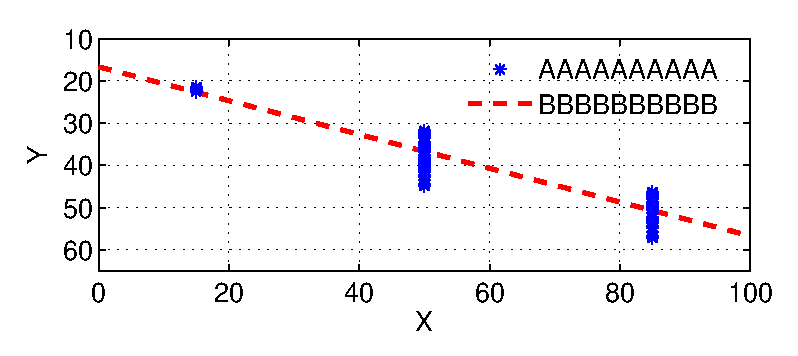
\includegraphics[width=\tamfig]{Figuras/ACAxDist.eps}
   \caption{Average channel attenuation depending on the distance between the transmitter and receiver of \ac{PLC} signals.}
   \label{Fig:ACAxDist}
\end{centering}
\end{figure}

Fig.~\ref{Fig:SenoJanelaZero} illustrates the variation of \ac{ACA} value of one \ac{PLC} outdoor channel. By comparing with the main signal magnitude ($60$~Hz in Brazil), these variations in ACA amplitude occurs in a time window centered at the instant time in which the \ac{LV-PDN} main signal crosses the zero. The observed average duration of the time window occupied by the abrupt \ac{ACA} variation of measured outdoor PLC channels was $T_{W^{120}} = 0.98$~ms, since the observed values ranged from 0.73~ms up to 1.40~ms. 
This \ac{ACA} alteration is related to the switching synchronized with the fundamental frequency of the loads connected to the electric power network. This abrupt and cyclic change in the \ac{ACA} has been reported in other papers for indoor \ac{PLC} channels \cite{Corripio2006, Oliveira2017}.

\begin{figure}[!htp]
\begin{centering}
    \psfrag{X}[Bc]{Time (ms)}    
    \psfrag{Y}[bc]{unscaled}
    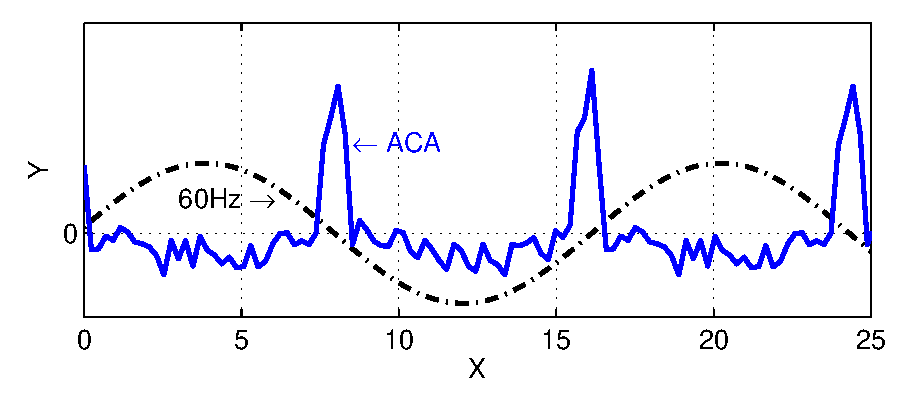
\includegraphics[width=\tamfig]{Figuras/SenoJanelaZero.eps}
    \caption{Temporal window containing the abrupt change of the ACA of the channel PLC outdoor due to zero crossing of the fundamental frequency of LV-PDN}
    \label{Fig:SenoJanelaZero}
\end{centering}
\end{figure}

\subsection{Average Channel Frequency Response}
The magnitude response of measured PLC channels, in terms of maximum, mean and minimum value, is depicted in Fig.~\ref{Fig:CFRmedia}. As can be seen, the mean value of the magnitude response of outdoor PLC channels exhibit a decay rate of, approximately, 0.4~dB/MHz. Furthermore, high attenuation is observed at the initial portion of the analyzed spectrum up to 1.7~MHz due to the action of the high-pass filter of the PLC coupler applied in the measurements. Fig.~\ref{Fig:CFRmedia} also shows a robust approach of the mean measured PLC channel attenuation response based on the mean square error criterion, given by
\begin{eqnarray} \label{eq-CFRmedia}
\widetilde{A}_f(f) = 0.391f+36.3 \   \  \mbox{[dB]},   
\end{eqnarray}
with $f$ given in MHz.

\begin{figure}[!htp]
	\begin{centering}
		\psfrag{X}[Bc]{Frequency em MHz}    
		\psfrag{Y}[bc]{ACFR (dB)}
		\psfrag{AAAAAAAAAA}[Bl]{Average}
		\psfrag{BBBBBBBBBB}[Bl]{Model}
		\psfrag{curva1}[Bl]{min}
		\psfrag{curva2}[Bl]{max}		
		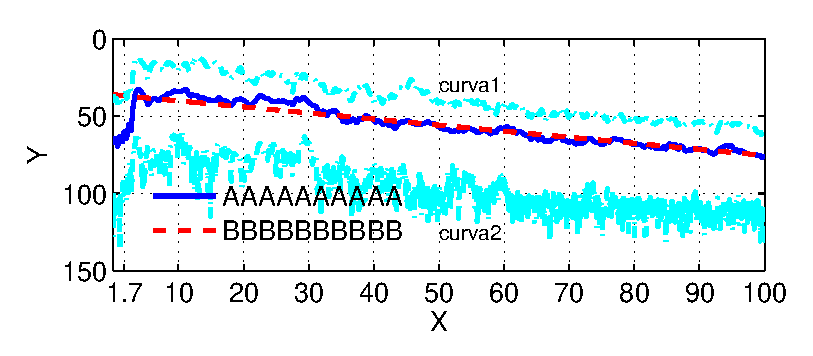
\includegraphics[width=\tamfig]{Figuras/CFRmedia.eps}
		\caption{Average channel frequency response of outdoor PLC channel measured in dB and its robust approach as a function of frequency.}
		\label{Fig:CFRmedia}
	\end{centering}
\end{figure}

\subsection{Temporal dispersion}\label{sec-rmsds}
The \ac{RMS-DS} statistics are indicated in Tab.~\ref{Tab:EstatisticasRMS}. As can be observed, the RMS-DS was smaller than $0.22$~ms in 90\% of the analyzed cases. 
\begin{table}[!htb]
\centering
\caption{Root mean squared delay spread statistics of outdoor PLC channel in milliseconds.}
\footnotesize  
\begin{tabular}{c|c|c|c|c|c|c}
\hline 
           &  Min    & Max    & Mean    & Std    & 90\% above    & 90\% below \\
\hline 
RMS-DS     & 0.13   & 0.30  &  0.19    & 0.30   & 0.16          & 0.22 \\
\hline
\end{tabular} \label{Tab:EstatisticasRMS}
\newline
\end{table}   

Fig.~\ref{Fig:RMSDS_CDF} shows the empirical \ac{CDF} of the RMS-DS. The RMS-DS presented values between 129.7~$\mu$s and 301.6~$\mu$s following, with good approximation, the inverse gaussian probability distribution ($\mu$ = 0.186993, $\lambda$ = 8.71957).
\begin{figure}[!htp]
\begin{centering}
    \psfrag{X}[Bc]{RMS-DS ($\mu$s)}    
    \psfrag{Y}[bc]{CDF}
    \psfrag{AAAAAAAAAA}[Bl]{Measured}
    \psfrag{BBBBBBBBBB}[Bl]{Inverse Gaussian}
    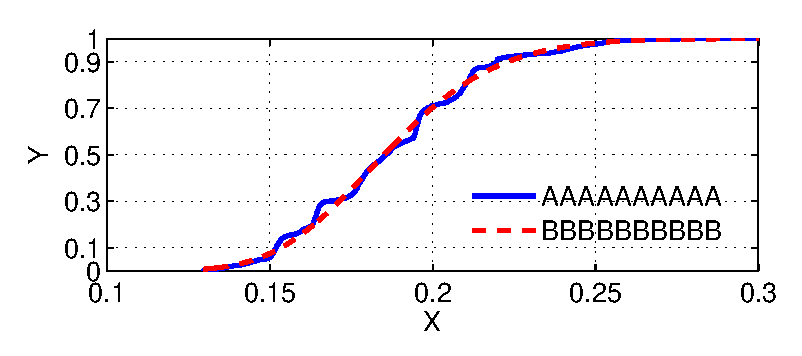
\includegraphics[width=\tamfig]{Figuras/RMSDS_CDF.eps}
    \caption{Cumulative distribution function of root-mean-square delay spread of the outdoor \ac{PLC} channel and the approaches by inverse gaussian distribution.}
    \label{Fig:RMSDS_CDF}
\end{centering}
\end{figure}


\subsection{Root Mean Squared Delay Spread versus Average Channel Attenuation}
The relation between ACA and RMS-DS in outdoor \ac{PLC} channel can be observed in Fig.~\ref{Fig:ACMxRMSDS}. This relation can be modeled by robust linear approach based on the mean square error criterion, given by   
\begin{eqnarray} \label{eq-ACMxRMSDS}
\sigma_{\tau} = - 0.01 \times1 0^{-2}A_f + 0.19 \   \  \mbox{[$\mu$s]},    
\end{eqnarray}
where $\sigma_{\tau}$ is the RMS-DS in microseconds.

\begin{figure}[!htp]
\begin{centering}
    \psfrag{X}[Bc]{ACA (dB)}    
    \psfrag{Y}[bc]{RMS-DS ($\mu$s)}
    \psfrag{AAAAAAAAAA}[Bl]{Average}
    \psfrag{BBBBBBBBBB}[Bl]{Model}
    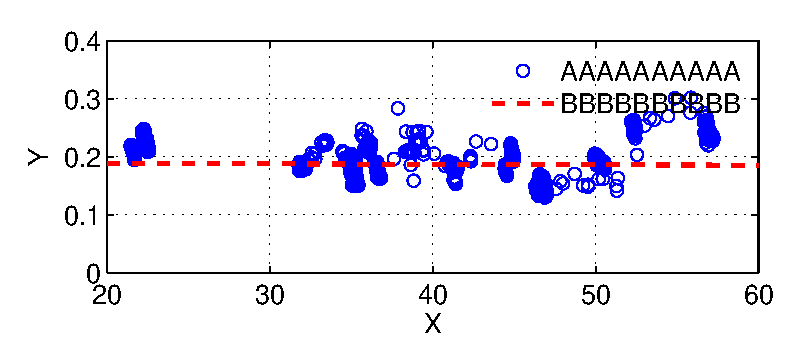
\includegraphics[width=\tamfig]{Figuras/ACGxRMSDS.eps}
    \caption{Variation of RMS-DS due to ACA.}
    \label{Fig:ACMxRMSDS}
\end{centering}
\end{figure}

\subsection{Coherence Bandwidth}\label{sec-bandadecoerencia}

The \ac{CB} statistics are indicated in Tab.~\ref{Tab:EstatisticasCB}, where it is observed that in 90\% of the analyzed cases  \ac{CB} is higher than 351.24~kHz.
\begin{table}[!htb]
\centering
\caption{Coherence bandwidth statistics for $\gamma = 0.9$ of outdoor PLC channel in kHz.}
\footnotesize 
\begin{tabular}{c|c|c|c|c|c|c}
\hline 
                  &  Min    & Max    & Mean    & Std     & 90\% above   & 90\% below \\
\hline 
CB                & 247.20  & 629.21 &  430.57 & 75.00   & 351.24       & 542.74 \\
\hline
\end{tabular} \label{Tab:EstatisticasCB}
\newline
\end{table} 

The empirical CDF of CB is shown in Fig.~\ref{Fig:BC_CDF}, when  $\gamma = 0.9$ is considered. In this case, CB varies from 247.2~kHz up to 629.2~kHz following, with good approximation, a inverse Gaussian probability distribution ($\mu$ = 430.57, $\lambda$ = 14,323.9).  
\begin{figure}[!htp]
\begin{centering}
    \psfrag{X}[Bc]{CB (kHz)}    
    \psfrag{Y}[bc]{CDF}
    \psfrag{AAAAAAAAAA}[Bl]{Measured}
    \psfrag{BBBBBBBBBB}[Bl]{Inv. Gaussian}
    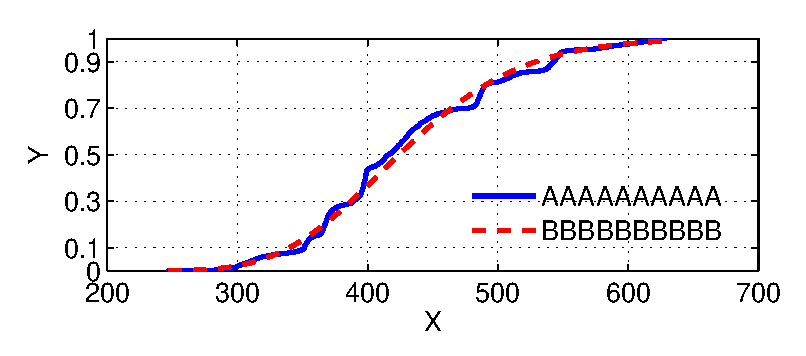
\includegraphics[width=\tamfig]{Figuras/BC_CDF.eps}
    \caption{Cumulative distribution function of coherence bandwidth of the outdoor PLC channel and the approaches by inverse gaussian and normal distribution.}
    \label{Fig:BC_CDF}
\end{centering}
\end{figure}
  
\subsection{Root Mean Squared Delay Spread versus Coherence Bandwidth}

The relationship between RMS-DS and CB can be verified in Fig.~\ref{Fig:RMSDSxBC}. The derived model was obtained through a robust approximation following a hyperbolic curve, which can be represented by
\begin{eqnarray} \label{eq-RMSDSxBC}
B_c^{0.9} = \frac{78.5}{\sigma_{\tau}},    
\end{eqnarray}
where $B_c^{0.9}$ refers to the CB when $\varphi=0.9$ in kHz and $\sigma_{\tau}$ is the RMS-DS in $\mu$s.

\begin{figure}[!htp]
\begin{centering}
    \psfrag{X}[Bc]{RMS-DS ($\mu$s)}    
    \psfrag{Y}[bc]{CB (kHz)}
    \psfrag{AAAAAAAAAA}[Bl]{Measured}
    \psfrag{BBBBBBBBBB}[Bl]{Model}
    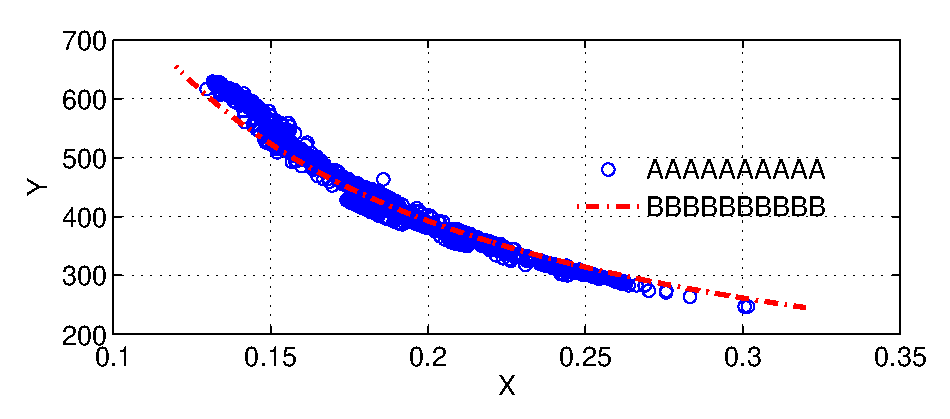
\includegraphics[width=\tamfig]{Figuras/RMSDSxBC.eps}
    \caption{RMS delay spread \emph{versus} coherence bandwidth ($\varphi = 0.9$).}
    \label{Fig:RMSDSxBC}
\end{centering}
\end{figure}

\subsection{Coherence time}\label{sec-tempodecoerencia} 
Fig.~\ref{Fig:TCmedio} illustrates the average evolution of the coherence index between analyzed Brazilian outdoor \ac{PLC} channels. As can be seen, the occurrence of some valleys in the coherence index are due to abrupt change of the \ac{CIR} that occurs in the passage through zero of the fundamental frequency of the electrical energy network.  
\begin{figure}[!htp]
\begin{centering}
    \psfrag{X}[Bc]{Temporal Separation (ms)}    
    \psfrag{Y}[bc]{$|\rho_h|$}
    \psfrag{AAAAAAAAAA}[Bl]{Average}
    \psfrag{BBBBBBBBBB}[Bl]{Measured}
    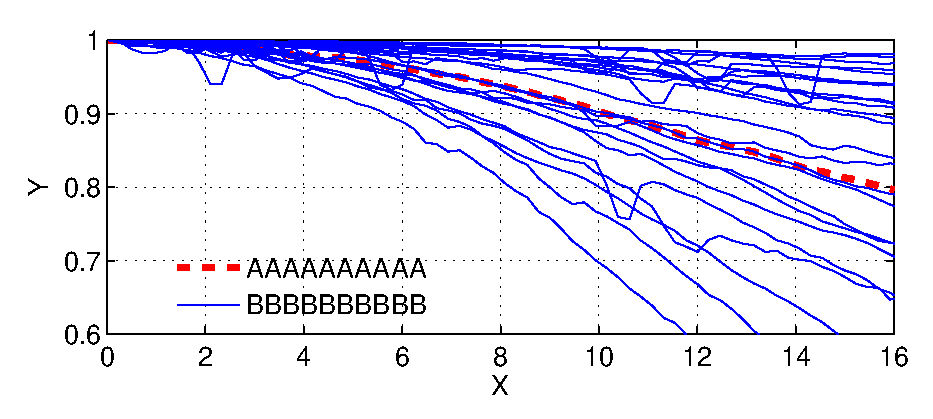
\includegraphics[width=\tamfig]{Figuras/TCmedio.eps}
    \caption{Average evolution of the coherence index between outdoor PLC channels.}
    \label{Fig:TCmedio}
\end{centering}
\end{figure}

Fig.~\ref{Fig:TC_CDF} depicts the cumulative distribution function of the \ac{PLC} channel coherence time. As can be seen,  only in 20\% of the analyzed cases the coherence time was less than approximately 2~ms for $\beta = 0.99$, and 5~ms for $\beta = 0.95$. 
\begin{figure}[!htp]
\begin{centering}
    \psfrag{X}[Bc]{Time (ms)}    
    \psfrag{Y}[bc]{CDF}
    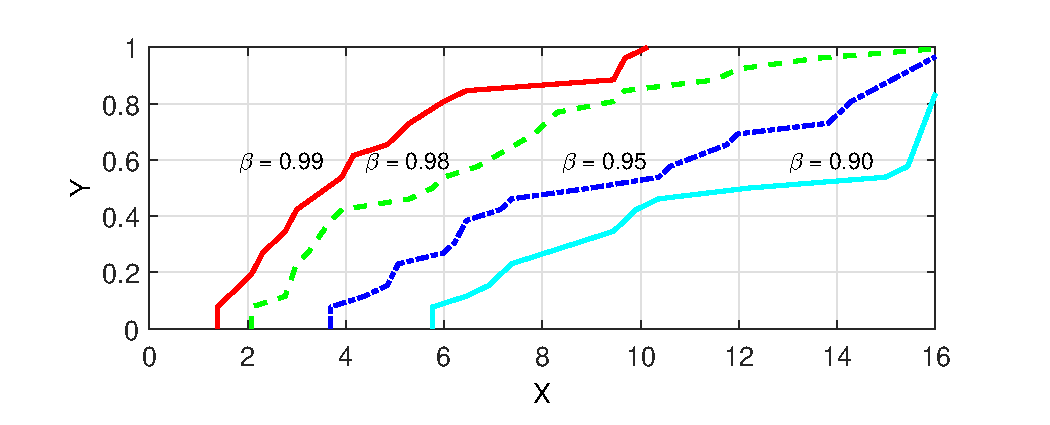
\includegraphics[width=3.8in]{Figuras/TC_CDF.eps}
    \caption{Cumulative distribution function of coherence time of outdoor PLC channel.}
    \label{Fig:TC_CDF}
\end{centering}
\end{figure}

The \ac{CT} statistics are indicated in Tab.~\ref{Tab:EstatisticasCT}, considering $\beta=\{0.90;0.95;0.98;0.99\}$. As can be observed, the coherence time observed from the measurement campaign was not lower than 1.38~ms and 5.76~ms, for $\beta=0.99$ and $\beta = 0.90$, respectively. The highest \ac{CT} value indicated in the TAB was limited by the storage capacity of the consecutive \ac{CFR}s of the measurement equipment (723 \ac{CFR}s) adopted in the measurement campaign.

\begin{table}[!htb]
\centering
\caption{Coherence time statistics of outdoor PLC channel in ms.}
\footnotesize 
\begin{tabular}{c|c|c|c|c|c|c}
\hline 
$\beta$    &  Min    & Max    & Mean    & Std     & 90\% above   & 90\% below \\
\hline 
0.99       & 1.38    & 10.14 &  4.50    & 2.70   & 1.59         & 9.49 \\
\hline
0.98       & 2.07    & $>$16.36 &  6.55    & 3.83   & 2.49         & 11.70 \\
\hline
0.95       & 3.69    & $>$16.36 &  9.84    & 4.56   & 4.10         & 15.27 \\
\hline
0.90       & 5.76    & $>$16.36 &  12.28   & 4.21   & 6.18         & 16.36 \\
\hline

\end{tabular} \label{Tab:EstatisticasCT}
\newline
\end{table}  

\subsection{Noise}\label{sec-ruido}
In this work, each measured noise group has $N_v=3,500.000$ samples and it is classified as background noise if all of its samples assume values less than $V_{\lim}$. Otherwise, that is, the measured noise group has some sample with an amplitude greater than or equal to $V_{\lim}$, it receives the classification of impulsive noise. Fig.~\ref{Fig:limiteDeciRuidos} illustrates the two classes of noise adopted to model the noise of \ac{LV-PDN} when $V_{\lim}=0.05$~V. In the Figure above the peak value of the noise amplitude did not exceed the decision threshold $V_{\lim}$, so this group of $N_v$ samples is classified as background noise. In the figure below, it is possible to identify that there are samples from the group where their amplitudes exceed the decision threshold, so the group is classified as impulsive noise. 
\begin{figure} [!htb]
    \begin{minipage}[b]{\linewidth}
    \psfrag{X}[Bc]{Samples}    
    \psfrag{Y}[bc]{Amplitude (V)}
    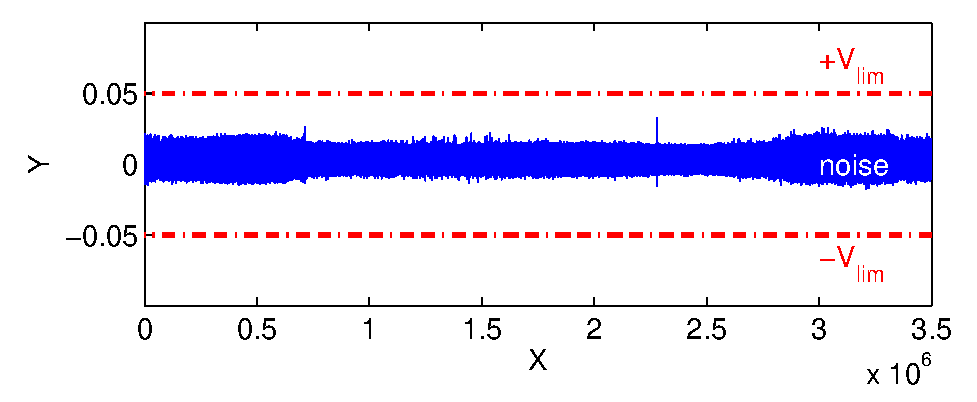
\includegraphics[width=\linewidth]{Figuras/limiteDeciRuidoRimpuls11.eps}
    \begin{center} \vspace{-.4cm}
    (a) Background noise.
    \end{center}
	\vfill
    \end{minipage} 
    \begin{minipage}[b]{\linewidth}
    \psfrag{X}[Bc]{Samples}    
    \psfrag{Y}[bc]{Amplitude (V)}
    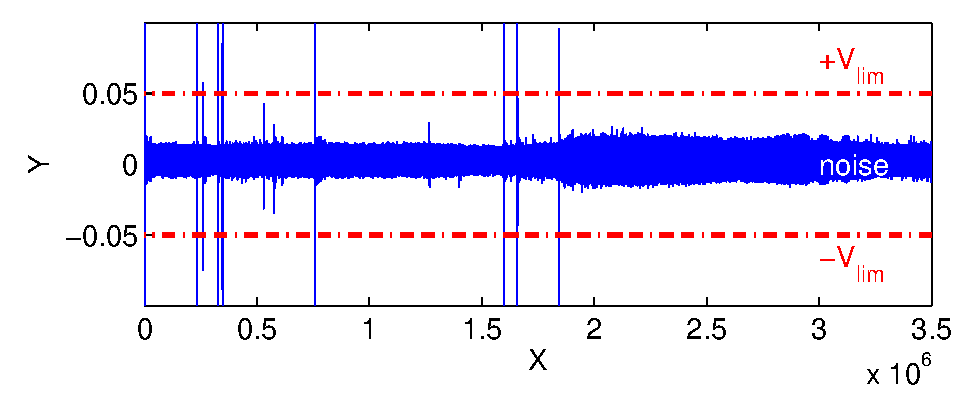
\includegraphics[width=\linewidth]{Figuras/limiteDeciRuidoRimpuls6.eps}
    \begin{center}\vspace{-.4cm}
    (b) Impulsive noise.
    \end{center}
    
    \end{minipage}
    \caption{Classification of the noise measured as a noise peak amplitude function  (a) background noise and (b) impulsive noise.}
    \label{Fig:limiteDeciRuidos}
\end{figure}

Fig.~\ref{Fig:PSDRuidoFundoImp} illustrates the PSD averaged of the two group of measured noise, background and impulsive noise, classified as described above. 
\begin{figure}[!htp]
\begin{centering}
    \psfrag{X}[Bc]{Frequency (MHz)}    
    \psfrag{Y}[bc]{PSD (dBV$^2$/Hz)}
    \psfrag{AAAAAAAAAA}[Bl]{impulsive}
    \psfrag{BBBBBBBBBB}[Bl]{background}
    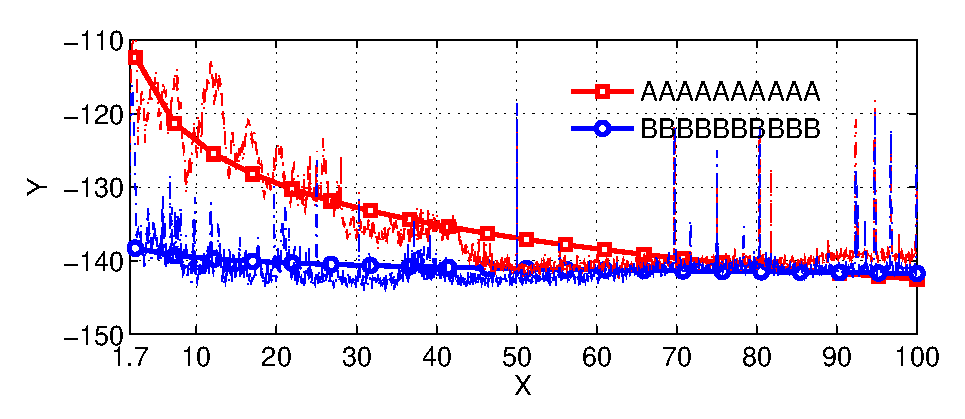
\includegraphics[width=\tamfig]{Figuras/PSDRuidoFundoImp.eps}
    \caption{Average PSD both background and impulsive noises of the low voltage electric power distribution networks and their respective models.}
    \label{Fig:PSDRuidoFundoImp}
\end{centering}
\end{figure}

The PSD of background and impulsive noise can be modeled by
\begin{eqnarray}\label{eq-psdOutdoor}
S_n(f) = a + b\log_{10}|f| \ \ \ \mbox{in dBV$^2$/Hz},  
\end{eqnarray}
where $a$ and $b$ are parameters dependent on the location of the measurements and $f$ is the frequency in MHz. The values of $a$ and $b$ that model the noise present in the Brazilian \ac{LV-PDN} when considering the band of frequency of 1.7~MHz up to 100~MHz are indicated in Tab.~\ref{Tab:ParamNoise}. 
\begin{table}[!htb]
\centering
\caption{Parameters for noise models}
\footnotesize 
\begin{tabular}{c|c|c}
\hline 
Type of Noise    & $a$ & $b$\\ 
\hline 
background & -137.5 & -2.1  \\
\hline
impulsive & -105.3 & -18.6  \\
\hline
\end{tabular} \label{Tab:ParamNoise}
%\newline
\end{table}

\subsection{Achievable data rate}
Thus, we have \ac{ADR} estimate of the outdoor \ac{PLC} channel equivalent of a frequency selective channel whose restrictions on the transmitted signal and additive noise are those described in this section. It was adopted $|H[k]|^2 = 10^{-5}$, $k=0,1,\ldots,N-1$, i.e, $\widetilde{A}_f(50\ \mbox{MHz}) \approx  50$~dB (Fig.~\ref{Fig:CFRmedia}). Fig. \ref{Fig:Capacidade} shows the achievable data rate of outdoor PLC in the presence both background and impulsive noise when considering the frequency band of 1.7-100 MHz.
\begin{figure}[!htp]
\begin{centering}
    \psfrag{X}[Bc]{PSD of transmitted signal (dBV$^2$/Hz)}    
    \psfrag{Y}[bc]{ADR (Mbps)}
    \psfrag{AAAAAAAAAA}[Bl]{impulsive}
    \psfrag{BBBBBBBBBB}[Bl]{background}
    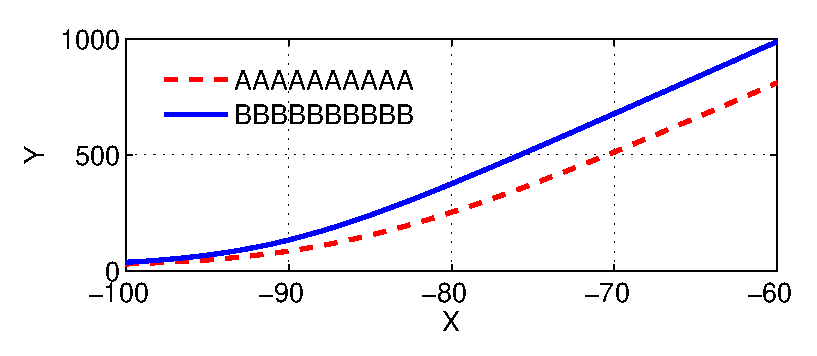
\includegraphics[width=\tamfig]{Figuras/Capacidade.eps}
    \caption{Achievable data rate of the outdoor \ac{PLC} channel in the presence both impulsive and background noise.}
    \label{Fig:Capacidade}
\end{centering}
\end{figure} 

Finally, the main parameters that aid in the characterization of Brazilian outdoor PLC channel are summarized in Tab.\ref{Tab:Estatisticas}.

\begin{table*}[!htb]
\centering
\caption{Brazilian outdoor PLC channel statistics}
\begin{tabular}{c|c|c|c|c|c|c|c}
\hline 
Parameters           & Min    & Max    & Mean     & Std     & 90\% above    & 90\% below & Distribution\\
\hline
$T_{W^{120}}$ [ms]   & 0.73   & 0.98   &  1.40    & 0.12    &  0.73         & 1.15       & \\
\hline
ACA [dB/m]          &        &        &  0.40    &         &               &            & \\
\hline
ACFR [dB/MHz]        &        &        &  0.40    &         &               &            & \\
\hline
RMS-DS [$\mu$s]      & 0.13   & 0.30   & 0.19     & 0.03    & 0.16          & 0.22       & Inv. Gaussian\\
\hline
CB$^{*1}$ [kHz]      & 247.2  & 629.2  & 430.6    & 75.01   & 351.24        & 542.74     & Inv. Gaussian\\
\hline
CT$^{*2}$ [ms]       & 2.07   & $>$16.3  & 6.55     & 3.83    & 2.49          & 11.70      & \\
\hline 
\end{tabular} \label{Tab:Estatisticas}
\newline
\begin{tabular}{ccccc}
Note 1: $\gamma = 0.9$ &  &Note 2: $\beta=0.98$ & & \\  
\end{tabular}
\end{table*}


\section{Conclusion}\label{sec-conclusao}
This work presented the results of a comprehensive measurement campaign with the aim of characterizing and modeling the Brazilian \ac{LV-PDN} as a means of data communication in the frequency band from 1.7~MHz up to 100~MHz.

Concerning the calculation of the coherence band and coherence time, it has been proposed to consider the outdoor \ac{PLC} channel as having scattering uncorrelated and stationary in the broad sense. This modeling proved to be feasible since the lowest coherence time of the \ac{PLC} outdoor channel found during the measurement campaign was 207~$\mu$s, which is much longer than 23,4~$\mu$s in which corresponds to the duration of the transmitted symbol. 

Statistical models that represent the RMS-DS and CB of the measured channels were presented. Also, the temporal window statistic and average gain variation that occur due to periodic cyclic variations in the frequency response of the \ac{PLC} channel was discussed at the first time.

Mathematical models, based on only two parameters, representing the background and impulsive noises present in \ac{LV-PDN} have been proposed.

Finally, the achievable data rate of the outdoor PLC channel in the presence both impulsive and background noise was estimated.
\section*{Acknowledgment}

The authors would like to thank, FINEP, FAPEMIG, CNPq, CAPES, P\&D
ANEEL, CEMIG, INERGE and Smarti9 for their financial supports.

\bibliographystyle{IEEEtran}
\bibliography{bib_tese}

\end{document}
